\documentclass[../main.tex]{subfiles}
\graphicspath{{\subfix{../images/chapter1/}}}
\begin{document}

\chapter{Introduction}

\section{Overview}
Electric circuits are really important. In a world filled with electronic devices and appliances, circuits are everywhere, from the smartphones we carry in our pockets everyday, to the cars we use to move around, or the complex power grid systems we rely on. Although all of the things previously mentioned vary greatly in a lot of ways, they all share the same basic electrical concepts and components.

\subsection{What are electric circuits?}
\begin{figure}[ht]
\centering
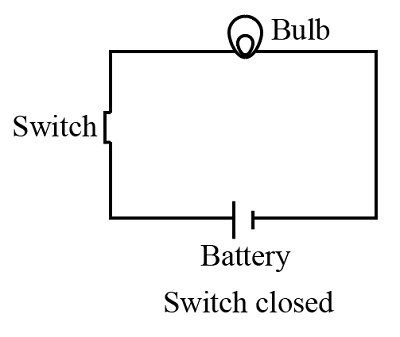
\includegraphics[scale=0.5]{images/chapter1/basic_circuit.png}
\caption{Basic electric circuit}
\label{fig:basic circuit}
\end{figure}
An electric circuit can be described as a closed path or a loop that acts as a continuous pathway for electrons to flow, this flow is what we call electric current. Circuits can be represented in many different ways. Essentially, all you need to have a circuit is a conductive material and a power source, you can then use the current of electrons flowing through the circuit to power any devices you want. A very simple example of a circuit is one which contains a battery, a wire and a light bulb, figure \ref{fig:basic circuit} demonstrates how such a circuit would look like.
Circuits are usually made up of several basic components, each component can be categorized as either: 
\begin{enumerate}
\item \underline{An active component}: which is An electric circuit element which can supply electric power to the circuit or power gain in the circuit. Examples of such components are:
\begin{itemize}
\item Batteries.
\item Amplifiers.
\item Transistor
\end{itemize}
\item \underline{A passive component}: a circuit element which can only absorb electrical energy and dissipates it in the form of heat or stores in either magnetic field or electric field. Examples include:
\begin{itemize}
    \item Resistors.
    \item Capacitors.
    \item Inductors.
\end{itemize}
\end{enumerate}
Each of these components can also be of different types each of which are more suited for different functions, for example transistors can be bipolar, junction, field-effect.



\subsection{Electric circuits’ impact on our lives}
Electric circuits form the fundamentals of modern day societies, they allow us to harness and control electricity and use it to make our lives easier. Many aspects of our day-to-day lives depend on them.
To really feel the impact of circuits on our lives, try to think about any electric device or appliance, without circuits these things would cease to exist, take for example the artificial lights that light up our nights, a thing we take for granted and completely depend on. Another example is computers. Computers are involved in almost everything in our lives, either directly by being a part of the device itself, or indirectly by being involved in the manufacturing process.



\subsection{Electric circuits educational challenge}
\subsubsection{Electric circuits education}
Thus far we have established the importance of electric circuits in our lives, and that should lead us to the following conclusion: in order to maintain the technological innovations and developments, we need a lot of people to have a professional understanding of how circuits work, how they are designed and built, and how they can be utilized properly. Luckily a lot of people have come to that conclusion many decades ago, and now students in schools and in \acrfull{stem} related university programs do study electric circuits to some extent.

\subsubsection{The challenge}
Students often find the topic of electric circuits to be a daunting or a complex topic to study, it is a topic often associated with the idea of being difficult. And that applies to both the theoretical side and the practical side of the learning process, it is a demanding topic that requires the student to have an understanding in multiple fields such as mathematics and physics. And even solutions such as circuits simulation programs most of them are old, not so user friendly, and require a level of proficiency with the program itself before a student can start using it. Latest studies suggest that students often find problems understanding topics such as current and voltage behavior in sequential and parallel circuits (Bowman et al., 2007)\cite{1}.

\subsubsection{Our proposed solution}
Our proposed solution to help circuit students of all levels is to make an educational game, the game would offer them an interactive gamified learning experience with a decent learning curriculum. The main goal is to guide students along a journey of building different circuits with different purposes, and along this journey the student will be learning about different components and different characteristics they possess, and how components connected together in a certain way could make a useful circuit.
A reason for why people like playing games and spend so much time doing it is that games are fun, entertaining and rewarding. And that will be a core focus for our game. A big part of the gamified learning experience is keeping students interested, and eager to continue completing more levels of the game, and that can be achieved by adhering to game design techniques, and having an educative yet enjoyable directory of available levels.


\section{Gamification and education}
\subsection{Gamification}
There have been a lot of different definitions for gamification with different perspectives from different authors. Dixon, Khaled, and Nacke suggested defining “gamification” as “the use of game design elements in non-game contexts”. van Grove(2011) \cite{2} ”Gamification is to change something that is not a game through a game or its elements.”. MacMillan (2011) \cite{3} ” Gamification, defined as the use of game mechanics, dynamics, and frameworks to promote desired behaviors”. So we could simply say that gamification is the systematic process of applying game mechanics to non-game contexts to make difficult tasks more enjoyable. 
\subsection{Gamification as an approach}
Gamification is not just a technology, it is a psychology. Of the many fields within psychology, behavior analysis has devoted itself to precision in the understanding of, and perhaps more importantly the control of human behavior. A consideration of the principles generated by behavioral psychologists might be useful in explaining how specific game design elements motivate and maintain user engagement, and knowledge of the principles and processes defined by behavioral psychologists can readily help in the design of more useful and engaging gamified experiences. 
To design a successful and enjoyable gamification, a deeper understanding not only of games and play but also of the processes through which it is possible to incentivize people to behave in an appropriate or a productive manner is needed. Gamification offers a way for engaging and interactive education; plus, gamification actually aids in memory. According to Foerde and Shohamy \cite{4}, during gamification learning, a strong hippocampal\footnote{Hippocampus is a complex brain structure embedded deep into the temporal lobe. It has a major role in learning and memory.} activation makes the content easier to remember and recall.

\subsection{Gamification purposes}
Purposes of gamification differ from one to another, as a sense of purpose is integral to the field and circumstances it is used in. Also the human experiences should be taken into account. We believe that the main purpose of gamification is helping people to move from one point to another in their lives whether it is used for personal growth, societal improvement or marketing engagement. Also one of the main purposes of gamification that should exist in each gamification process is inspiring the users, giving them the motivation and encouraging them gracefully, effortlessly leading them into a steady stream of knowledge and experience, as successful gamification will tap into the user’s intrinsic motivation\footnote{Anything at all that makes you feel good within yourself is fueled by intrinsic motivation.}.
\subsection{Real impact of gamification}
According to a gamification survey made by TalentLMS which focused on productivity, motivation, and gamification for employee engagement. 83\% of those who receive gamified training feel motivated, while 61\% of those who receive non-gamified training feel bored and unproductive. 89\% believe they’d be more productive if their work was more gamified. \cite{5}
\begin{figure}[ht]
\centering
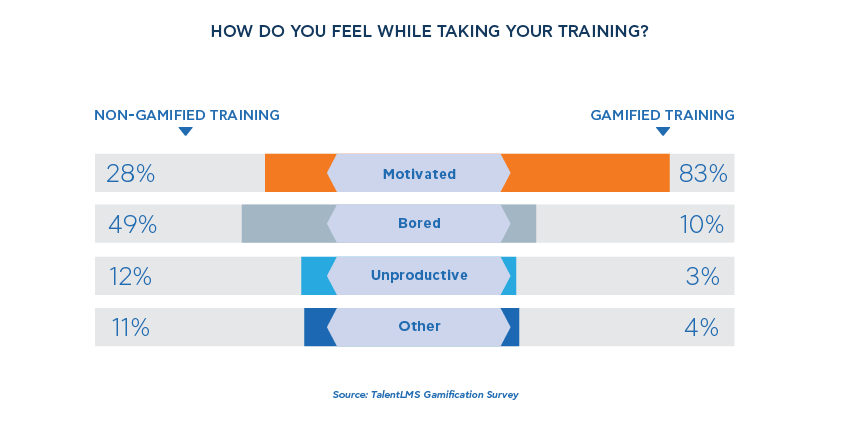
\includegraphics[scale=0.5]{images/chapter1/TalentLMS_Survey.png}
\caption{TalentLMS Gamification Survey}
\label{fig:TalentLMS gamification survey}
\end{figure}

\subsection{A brief history on gamification}
The gamification field as we know it started in late 2010, and it took its roots in the idea of using game elements and game designs in non-game contexts to reach various goals while increasing user engagement and motivation. Although the term has only been around for about a decade. History has witnessed numerous different things that have come together to form the rising industry of gamification. 
In 1896, Sperry \& Hutchinson (S\&H) made a meaningful step in the use of gamification; the company launched a stamp business. The number of S\&H stamps that customers collected from grocery stores, gas stations, and other businesses varied depending on how much money those customers spent on their products. The clients could then trade in their stamp collections for goods like various housewares. For educational purposes, games such as The Oregon Trail and Lemonade Stand were produced in the 1970s. In the 1980s, more efforts to use gamification for education were made. 
Gamification has an exciting future. This field has the potential to save industries millions by simulating training in an immersive and realistic environment that increases motivation and engagement. Gamification can generate learning and growth results that are better to those from any other strategy we have used in the past if it is implemented properly. It's time to take advantage of modern technology and our understanding of how the brain functions to improve performance and outcomes in a variety of contexts. A significant step in the right direction is being achieved through gamification \cite{6}, \cite{7}.
\begin{figure}
     \centering
     \begin{subfigure}[b]{0.3\textwidth}
         \centering
         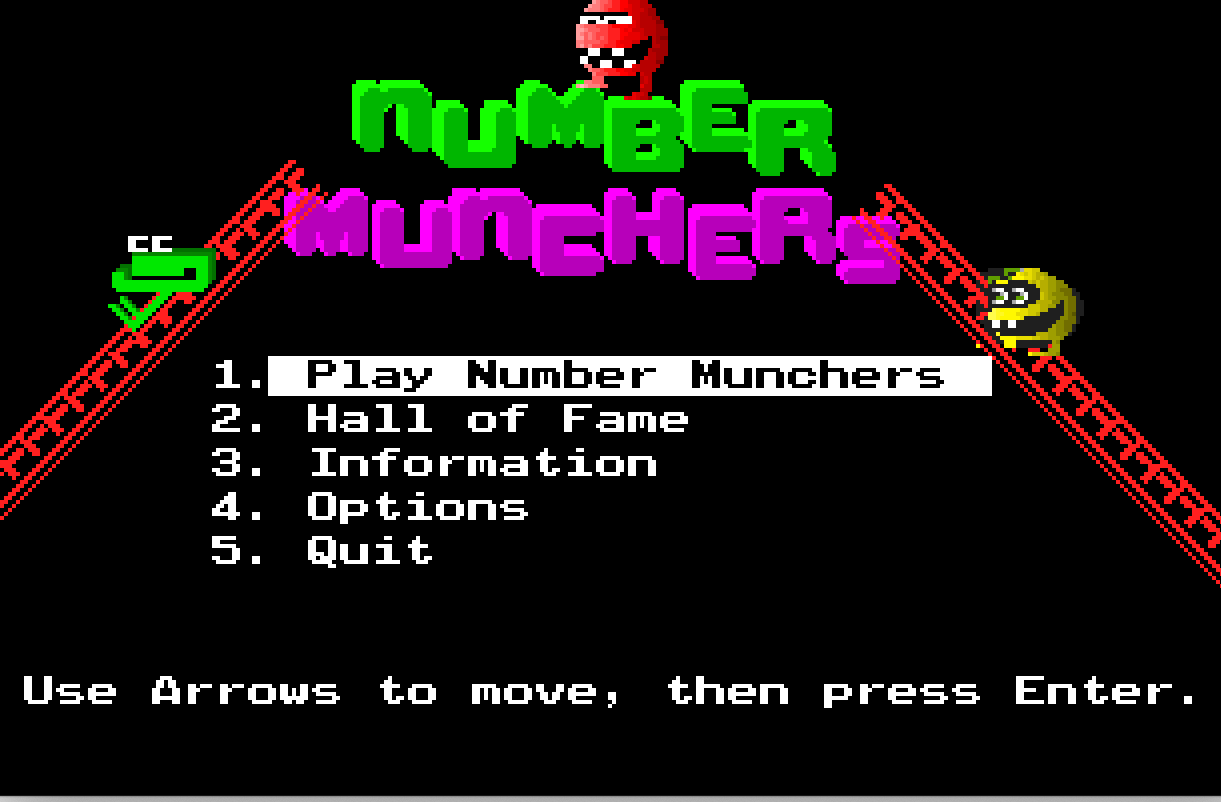
\includegraphics[width=\textwidth]{images/chapter1/old_games/number_munchers.png}
         \caption{Number Munchers (1986)}
         \label{fig:Number Munchers (1986)}
     \end{subfigure}
     \hfill
     \begin{subfigure}[b]{0.3\textwidth}
         \centering
         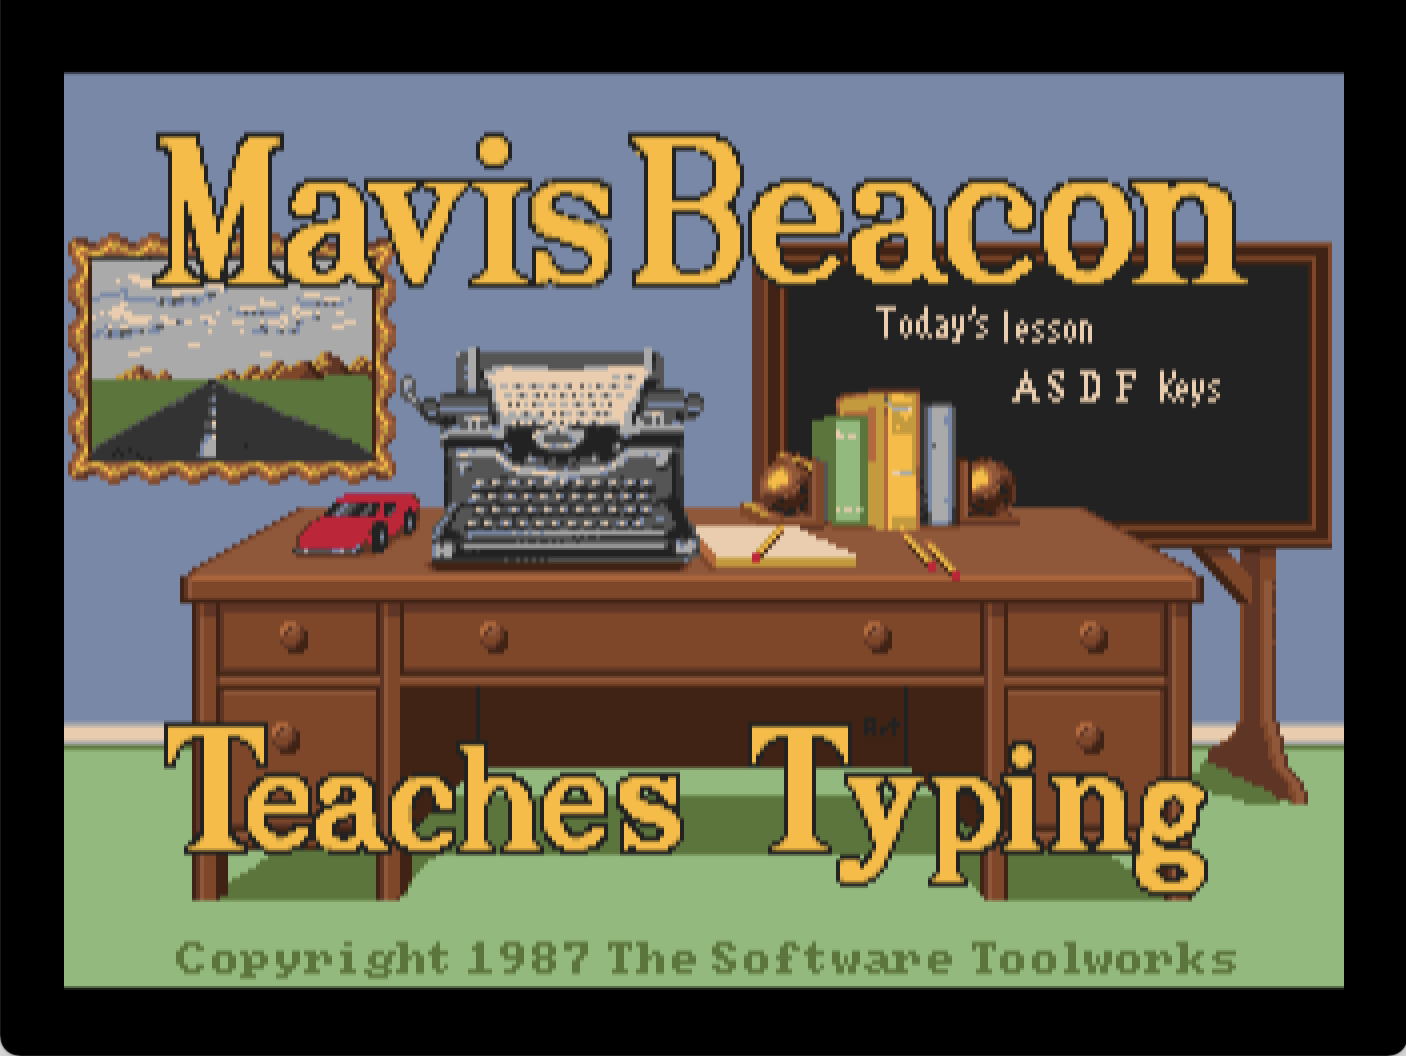
\includegraphics[width=\textwidth]{images/chapter1/old_games/MavisBeaconTeachesTyping.png}
         \caption{\raggedright Mavis Beacon Teaches (1987)}
         \label{fig:Mavis Beacon Teaches (1987)}
     \end{subfigure}
     \hfill
     \begin{subfigure}[b]{0.3\textwidth}
         \centering
         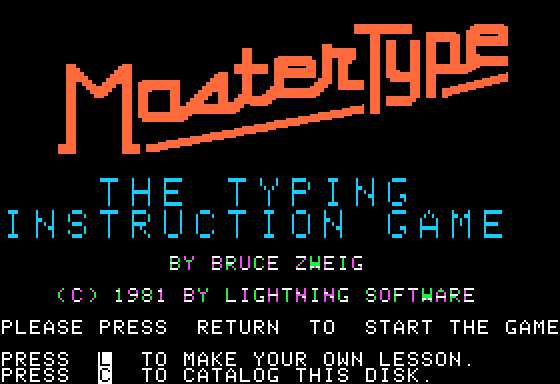
\includegraphics[width=\textwidth]{images/chapter1/old_games/MasterType.png}
         \caption{MasterType (1981)}
         \label{fig:MasterType (1981)}
     \end{subfigure}
        \caption{Old educational games}
        \label{fig:Old educational games}
\end{figure}

\subsection{Educational gamification}
Many educators face problems related to engagement and concentration of their students in their classrooms. These problems are not something new through generations, educators tried solving these problems using motivational and learning  strategies, however its effect did not last long as something in this environment fails to engage the students. The fun and playful nature of the game can be a good solution. 
Educational gamification proposes the use of game-like rule systems, player experiences and cultural roles to shape learners’ behavior, as it is an approach that seeks to motivate students and inspire them to learn, understand and concentrate easily. Understanding the role of educational gamification, means understanding the circumstances of the game elements that can drive learning behavior.
\begin{figure}[ht]
\centering
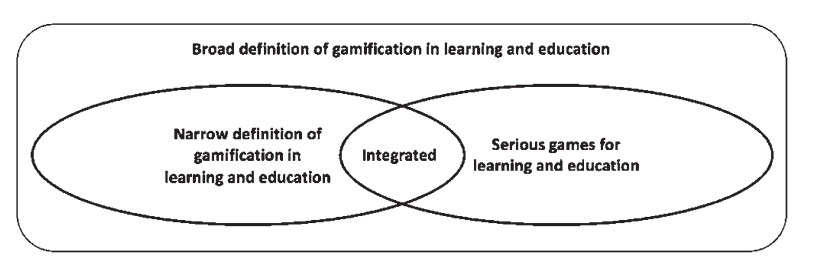
\includegraphics[scale=0.5]{images/chapter1/Broad definition of gamification in learning and education.png}
\caption{Broad definition of gamification in learning and education}
\label{fig:Broad definition of gamification in learning and education}
\end{figure}

\subsection{Motivation and engagement}
Motivation and engagement are concepts that are often used within the context of gamification. The properties of motivation and engagement are very complex as there are so many intertwined factors that can influence them. The quality of motivation and engagement needs to be understood. The motivation has two components (energy and direction), and engagement can be understood as the directional expression of motivation: when we direct our energy toward something or someone, engagement is observed. Engagement is not synonymous with motivation but is the behavioral expression of a motivated state.
Self-determination theory (Deci and Ryan 1985, 2000) \cite{8} suggests that the key to building successful gamification applications largely rests in:
\begin{enumerate}
    \item Understanding the energy that fuels our behavior.
    \item The various forms such energy can take.
    \item The ways in which we can apply this knowledge in the development of strategies, designs, and techniques to optimize the quality of motivational energy to achieve gamification’s goals.
\end{enumerate}
Which allows students to engage more in education through playing a game and having competition between themselves \cite{9}.

\subsection{The effect of gamification on students}
According to the International Journal of Education and Learning Systems \cite{10}, during the winter semester of the academic year 2016–2017, a study was carried out in which 20\% of ZSEM\footnote{Zagreb School of Economics and Management} undergraduate students took part. Eighty percent of the students who responded to the survey stated they were using gamification in at least one class. Students rated their happiness with the use of gamification in their courses on a scale ranging from 1 to 5. Of those, 67\% gave it a 5, 26,8\% gave it a 4, barely 5,2\% gave it a 3, and only one student expressed dissatisfaction\footnote{Student satisfaction in using gamification in class}.
90\% of students gave gamification a rating of 4 or 5 when asked how much it motivated them to attend lectures. Also, 86\% of students said that gamification improved their grades. Additionally, the majority of students concur that gamification needs to be included in the majority of the courses. Students showed their support for gamification in class in open responses because it helps them review their lectures through entertaining games and gives them more motivation.
\begin{figure}[ht]
\centering
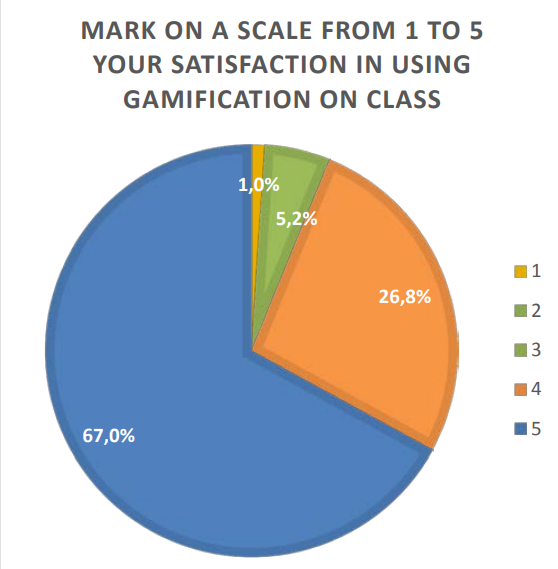
\includegraphics[scale=0.3]{images/chapter1/Students mark their satisfaction from 1 to 5 using gamification in class.png}
\caption{Students mark their satisfaction from 1 to 5 using gamification in class}
\label{fig:Students mark their satisfaction from 1 to 5 using gamification in class}
\end{figure}


\section{Game development}
\subsection{What is game production (development)?}
Game production, or as it’s more commonly referred to, game development\footnote{‘Game development’ is also often used to refer to all implementation-related tasks, like programming, algorithm design, etc… For the rest of this document, ‘game development’ will be used to refer to the whole production unless otherwise is specified.}, is the process of creating a video game (or any kind of game for that matter). It involves a tight combination of art and science, involving artistic creation skills, design, programming, engineering, testing, and possibly many more depending on the type of the game being developed. Long before its commercialization and the game industry becoming a ~\$200 billion industry, game development began around the 1950s on mainframe computers, until the first generations of commercial game consoles and arcade games became popular around the end of the 20th century. Nowadays, there are countless game studios ranging from a single developer to an international team dispersed across the globe, creating massively distributed multiplayer games, or singleplayer AAA titles comparable in production size and budget to Hollywood blockbusters. What exactly happens behind the scenes though? Why do games need that large of a team and wide skill-set?

\subsection{What is game design?}
Game design is a major sub-process of game development. It is concerned with defining the rules of games. What restrictions are there? What can the player do? How can they do it? What can't they do? What's their goal? How do they win? How do they lose? Is the game too easy? Too hard? Is this weapon too powerful? Is the game too simple? Too complex? What assumptions about the player's background does the game make? What experiences is it trying to convey? Does the game have a purpose besides entertainment? Game designers aim to define, prototype, communicate, and document the answers to all these questions and many more.
\subsubsection*{\underline{Normal (classic) game design vs video game design}}
Classic games were technologically restricted, that is, there was a lot that they couldn't do. They had to compensate for the lack of technology through game theory and game design, restriction forces creativity. A lot of the concepts used today in game design are borrowed from classic games. 


\subsection{Why is game design important for gamification?}
Gamification aims to make an otherwise dull experience tolerable, if not desirable. Good game design must be practiced, otherwise either the essence of the topic will be lost (preserve the essence of the topic), or the experience will just be dull, or even leaving a negative impression on the topic.


\subsection{The game development team roles (and other stakeholders)}
A lot goes into bringing a game to life, making game development and production a process that can take years, sometimes with teams into the hundreds depending on scope and budget. Here is a list of some of the core roles involved in game development \cite{12}, \cite{13}.
\subsubsection{Game designers}
\begin{figure}[ht]
\centering
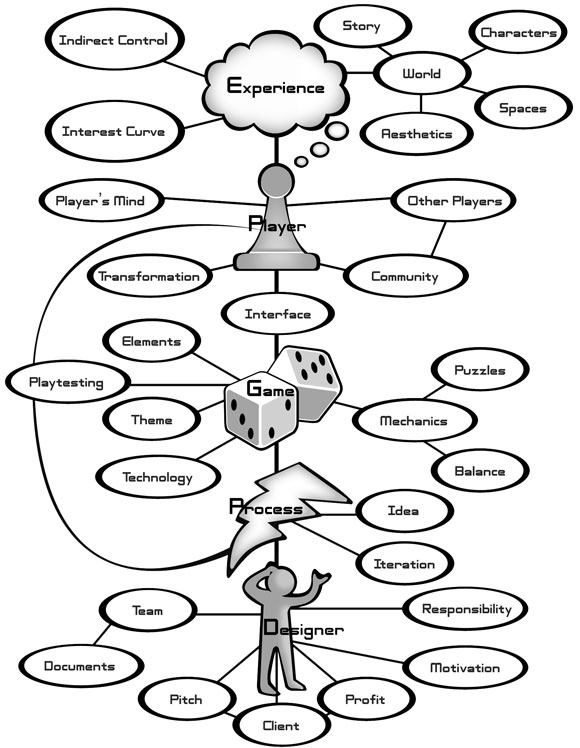
\includegraphics[scale=0.45]{images/chapter1/The Art of Game Design: A Book of Lenses, Second Edition: Chapter 34.png}
\caption{Schell, J. The Art of Game Design: A Book of Lenses, Second Edition: Chapter 34 (Complete game design map)}
\label{fig:Schell, J. The Art of Game Design: A Book of Lenses, Second Edition: Chapter 34 (Complete game design map)}
\end{figure}
Game designers handle creative elements of the game. This can include (but isn’t limited to) storyline creation, character definitions, game rules, goals and challenges. Anyone involved in the game’s development and responsible for making decisions, be it small or big, can also be considered a game designer. Game design requires both creative and technical competence; game designers may need to be artistic, possess creative and technical writing skills, as well as basic programming/scripting skills. In “The art of Game Design” by Jesse Schell, he suggests that any skill that you have can be (and will be) relevant to game design. These skills can be: animation, anthropology, architecture, brainstorming, business, cinematography, communication, creative writing, economics, engineering, games, history, management, mathematics, music, psychology, public speaking, sound design, technical writing, visual arts, and many more \cite{14}.
\subparagraph*{\underline{Key game designer roles}}
\begin{itemize}
    \item Lead designer
    \item Content designer
    \item Game mechanics designer
    \item Game rules designer
    \item Level designer (often a dedicated role due to importance and high workload)
    \item Environment designer
    \item System designer
    \item Game writer (story-line, characters, back-stories, lore, dialogue, etc…)

\end{itemize}
\subsubsection{Game programmers and engineers}
\subsubsection{Game artists}
Game development is an artistic production as much as it is a technical production. This group is responsible for bringing life to the game through colors,\acrfull{vfx}, animated \acrshort{3d} models, musical compositions, and much more. Game artists specializations are vast: character design, architecture and landscapes, lighting, modeling, special effects, texturing, and animation.
\subparagraph*{\underline{Key game artist roles}}
\begin{itemize}
    \item Character artists
    \item Concept artist
    \item Environment artists
    \item Asset artist
    \item Technical artist
    \item \acrshort{3d} model artist
    \item Animator
    \item \acrfull{sfx} artist
    \item Composer
\end{itemize}


\subsubsection{Some other stakeholders}
Larger scale games are not limited to the roles mentioned, and each game may outsource or dedicate internal talent to other unexpected fields as per need. Some more stakeholders in the game development industry may be (but not limited to):
\begin{itemize}
    \item \acrfull{qa} testers
    \item Project managers
    \item Game publishers \& distributors
    \item Creative directors
    \item Domain-specific/research consultants
    \item Localization teams
\end{itemize}

\subsection{Puzzle Design}
\subsubsection{Common definitions of a puzzle, and historic context}
A puzzle, in general, is a problem, game, or toy that tests a person’s problem solving skills in a given field or topic. A puzzle game is a game that focuses on challenging the player through logical thinking, as opposed to action or adventure \cite{15}.

\subsubsection{What is puzzle design?}
In order for a puzzle game to be successful, it needs to balance between difficulty, and reward. However, puzzle design is not just a matter of putting together a sequence of levels of increasing complexity; most puzzle games rely on logic in addition to another skill that the game either teaches the player or assumes they understand (in our case, electric circuit design). 

\subsubsection{How puzzle games are different from normal games (and what makes puzzle designers special)}
Puzzle game design differs from normal game design for multiple reasons; for one, the target audience is different, and for another, it’s much easier to design a frustrating experience when the action elements of video games are taken out. Puzzle designers might need to possess special skills, such as exceptional logical thinking or game theory knowledge for puzzles combinatorial in nature. In our case, out puzzles are circuit-based, and will require (from the designer’s perspective) a good handle on electric circuits, alongside standard successful puzzle game elements such as \cite{16}:
\begin{itemize}
    \item The game has a central mechanic that is easy to understand, but hard to master.
    \item The game should provide the player with all the information they need to complete the level, and understand the concept it’s teaching.
    \item Allow for the player to experiment, and get feedback on wrong solutions.
    \item Maintain balance between difficulty so that the player stays engaged, while making sure not to frustrate the player.
\end{itemize}

\subsubsection{Relation between education, learning,  puzzles, and circuits}
Putting together a circuit to satisfy a specific function is a puzzle; given a 5V battery, 3 100Ω resistors, and a standard red \acrshort{led}, how do you put together a circuit such that the LED is at highest brightness? How about the lowest brightness? What configurations could burn the LED out? These kinds of questions are puzzles in their nature, and the metaphor easily extends to other fields of education as well, not just electric circuits. Education as a learning approach, can be extended with engaging gamified experiences through puzzle games, that aid understanding, and facilitate an accessible way of experimentation, at lower costs and no risks.




\section{Problem definition}
\subsection{Challenges encountered by students when learning about electric circuits}
Most students regardless of their scientific level often find the idea of learning about circuits a very intimidating one, it is a topic that has been discussed and researched many times. Students from all levels may find difficulties in understanding topics such as voltage, current, and how these properties are affected by different components in a circuit. This can be seen for example in the research administered by Carol Bowman and Gordon J. Aubrecht, II \cite{1}, they found that students find the concept of voltage very confusing, and that is due to the fact that students first start by learning about current, then when they start learning about voltage they apply the idea of flow which applies to current, as a result students start confusing the two concepts together, and that it is despite careful texts which attempt to clarify the difference among the two.
Another challenge that students face nowadays is their very short attention spans. Students need something engaging and entertaining to keep them interested, traditional methods such as long lectures, and large textbooks, while informative, but they lack the attention grabbing element, students get bored and lose interest. According to Neil A. Bradbury \cite{17} several institutions have brought down the length of lectures to only 15 minutes. This is based on the belief that a lecture any longer than 15 minutes is not going to be effective for students.
Traditional techniques of circuit analysis do not provide students with the required skills for dealing with electric circuits effectively, students need to develop an intuition when analyzing circuits (Fino, 2018) \cite{18}.

\subsection{The materials available are geared towards professionals}
Many of the materials available to students are complex and require mastery of prerequisite skills such as mathematics and physics, surely there is an argument to be made for such materials, as they actually can be helpful for professionals as well as provide readers with a deeper understanding and intuition about the subject. But they aren’t particularly very helpful for beginner students trying to make their way through. As a matter of fact they can be confusing and discouraging, as they require the students to dedicate a long period of time to understanding how to effectively make use of the information presented, thus creating a barrier of entry. According to the authors of Should Textbooks Challenge Students? \cite{19}, not all students can learn at the same pace, therefore textbooks should provide an average challenge that can suit all students. 
According to (D. Sangam and B. K. Jesiek, 2015) \cite{20}, textbooks on electric circuits often lack important conceptual features, and that can pose a problem for beginners approaching the subject.

\subsection{Physical laboratories aren’t enough}
Available electric circuits courses usually rely only on textual materials to explain the subject, and while this kind of material is unquestionably important, it is not enough. Since electric circuits require practical and hands-on experience, some courses incorporate some form of hands-on practice through laboratories, according to Bayrak, Kanli, and İngeç \cite{21}, students learn information best when they can see the concepts and processes at work in the real world, but it’s not often that students can be surrounded by the real thing as it can be dangerous or inconvenient, that’s why stimulated environments such as laboratories are utilized. Although laboratories have their benefits, but they also come with limitations such as:
\begin{itemize}
    \item Components and tools being expensive to provide for every single student.
    \item Difficulty in managing a large number of students in the classroom.
    \item It takes too much time for teachers to plan such activities.
\end{itemize}
One method for overcoming those limitations would be to rely more on digital means for providing students with those stimulated environments, such as computer simulation programs. Simulation programs offer a variety of electrical components available for the student to use them in a circuit. There are also a lot of free and open source versions of such programs.

\subsection{Simulation programs aren’t beginner friendly}
\begin{figure}[ht]
     \centering
     \begin{subfigure}{0.25\textwidth}
         \centering
         
\includegraphics[width=\textwidth]{images/chapter1/NI Multisim.png}
         \caption{NI Multisim}
         \label{fig:NI Multisim logo}
     \end{subfigure}
     % \hfill
     \begin{subfigure}{0.25\textwidth}
         \centering
         
\includegraphics[width=\textwidth]{images/chapter1/LTSpice.jpg}
         \caption{LTspice}
         \label{fig:LTspice logo}
     \end{subfigure}
        \caption{Popular circuit simulation software programs}
        \label{fig:Logos of popular circuit simulation software programs}
\end{figure}
According to Jaakkola, Nurmi, and Veermans \cite{22}, students can gain better understanding about electric concepts when they combine both the real hands-on circuit experience, and also the use of computer circuit simulation programs. And that is great but usually circuit simulation programs aren’t beginner friendly and they require the understanding of their own notation, for example SPICE based simulators support their own unique commands. In addition to this most \acrshort{gui}-based SPICE simulators are outdated and hard to work with, not to mention the lack of convenient clear documentation or tutorials on how to make proper use of the software.
According to (Alasdoon, A. \& P.W.C, Prasad \& Beg, Azam \& Chan, A.., 2013) \cite{23}, commercial circuit simulators are great for use by professionals. But when it comes to students these programs have many disadvantages mainly because they are designed for commercial purposes and for the professional market. For example they might not have the basic simple functionalities that students require to finish their tasks, which might result in students getting confused. 

\end{document}